\documentclass[10pt,letterpaper]{article}
\usepackage[top=0.85in,left=2.75in,footskip=0.75in]{geometry}
\usepackage[utf8x]{inputenc}
\usepackage{setspace}
\usepackage{changepage}
\usepackage{amsfonts,amsmath, amsthm}
%\usepackage{geometry}
\usepackage{url}
\usepackage{appendix}
\usepackage{hyperref,nameref}
% textcomp package and marvosym package for additional characters
\usepackage{textcomp,marvosym}

% cite package, to clean up citations in the main text. Do not remove.
\usepackage{cite}

\usepackage{array}
% create "+" rule type for thick vertical lines
\newcolumntype{+}{!{\vrule width 2pt}}

% create \thickcline for thick horizontal lines of variable length
\newlength\savedwidth
\newcommand\thickcline[1]{%
  \noalign{\global\savedwidth\arrayrulewidth\global\arrayrulewidth 2pt}%
  \cline{#1}%
  \noalign{\vskip\arrayrulewidth}%
  \noalign{\global\arrayrulewidth\savedwidth}%
}

% \thickhline command for thick horizontal lines that span the table
\newcommand\thickhline{\noalign{\global\savedwidth\arrayrulewidth\global\arrayrulewidth 2pt}%
\hline
\noalign{\global\arrayrulewidth\savedwidth}}
% ligatures disabled
\usepackage{microtype}
\DisableLigatures[f]{encoding = *, family = * }
\usepackage{subcaption}
\doublespacing
% Text layout
\raggedright
\setlength{\parindent}{0.5cm}
\textwidth 5.25in 
\textheight 8.75in

% Bold the 'Figure #' in the caption and separate it from the title/caption with a period
% Captions will be left justified
\usepackage[aboveskip=1pt,labelfont=bf,labelsep=period,justification=raggedright,singlelinecheck=off]{caption}
\renewcommand{\figurename}{Fig}
\usepackage{graphicx}
\usepackage[right]{lineno}
\usepackage[table]{xcolor}
\makeatletter
\renewcommand{\@biblabel}[1]{\quad#1.}
\makeatother



% Header and Footer with logo
\usepackage{lastpage,fancyhdr,graphicx}
\usepackage{epstopdf}
%\pagestyle{myheadings}
\pagestyle{fancy}
\fancyhf{}
%\setlength{\headheight}{27.023pt}
%\lhead{\includegraphics[width=2.0in]{PLOS-submission.eps}}
\rfoot{\thepage/\pageref{LastPage}}
\renewcommand{\headrulewidth}{0pt}
\renewcommand{\footrule}{\hrule height 2pt \vspace{2mm}}
\fancyheadoffset[L]{2.25in}
\fancyfootoffset[L]{2.25in}
\lfoot{\today}


\title{Parameter estimation of the transmission probabilities of the 2015-2016 Zika outbreaks in the geopolitical regions of Brazil}
\author{}
\date{}


\begin{document}
\vspace*{0.2in}

% Title must be 250 characters or less.
\begin{flushleft}
{\Large
\textbf\newline{Parameter estimation of the transmission probabilities of the 2015-2016 Zika outbreaks in the geopolitical regions of Brazil} % Please use "sentence case" for title and headings (capitalize only the first word in a title (or heading), the first word in a subtitle (or subheading), and any proper nouns).
}
\newline
% Insert author names, affiliations and corresponding author email (do not include titles, positions, or degrees).
\\
Mugdha Thakur\textsuperscript{1*},
Baltazar Espinoza\textsuperscript{1},
Brian Klahn\textsuperscript{1},
Stefan Hoops\textsuperscript{1}
% Name5 Surname\textsuperscript{2\ddag},
% Name6 Surname\textsuperscript{2\ddag},
% Name7 Surname\textsuperscript{1,2,3*},
% with the Lorem Ipsum Consortium\textsuperscript{\textpilcrow}
\\
\bigskip
\textbf{1} Biocomplexity Institute and Initiative, University of Virginia, Charlottesville, Virginia, USA
\\
% \textbf{2} Affiliation Dept/Program/Center, Institution Name, City, State, Country
% \\
% \textbf{3} Affiliation Dept/Program/Center, Institution Name, City, State, Country
% \\
\bigskip

% Insert additional author notes using the symbols described below. Insert symbol callouts after author names as necessary.
% 
% Remove or comment out the author notes below if they aren't used.
%
% Primary Equal Contribution Note
%\Yinyang These authors contributed equally to this work.

% Additional Equal Contribution Note
% Also use this double-dagger symbol for special authorship notes, such as senior authorship.
%\ddag These authors also contributed equally to this work.

% Current address notes
%\textcurrency Current Address: Dept/Program/Center, Institution Name, City, State, Country % change symbol to "\textcurrency a" if more than one current address note
% \textcurrency b Insert second current address 
% \textcurrency c Insert third current address

% Deceased author note
%\dag Deceased

% Group/Consortium Author Note
%\textpilcrow Membership list can be found in the Acknowledgments section.

% Use the asterisk to denote corresponding authorship and provide email address in note below.
* mat3kk@virginia.edu

\end{flushleft}
% Please keep the abstract below 300 words
\section*{Abstract}



% Please keep the Author Summary between 150 and 200 words
% Use first person. PLOS ONE authors please skip this step. 
% Author Summary not valid for PLOS ONE submissions.   
\section*{Author summary}

\linenumbers
%\maketitle

%\begin{abstract}
    
%\end{abstract}


\section*{Introduction}
Zika virus (ZIKV) disease, although symptomatically mild, may cause severe morbidity due to microcephaly and other congenital and pregnancy problems, along with the suspected cases of Gullian-Barre Syndrome, brain and spinal cord swelling and blood disorders \cite{paixao2016history,da2017neurologic}. ZIKV, a flavivirus, can spread by the bite of \textit{Aedes} mosquitoes, through sexual contact and blood transfusions and can be passed to the fetus from an infected pregnant woman. ZIKV currently has no treatment or vaccine. Having critical associated morbidity and multiple transmission pathways, these factors lead to ZIKV's controls to heavily rely on the population and the vector management.

The first confirmed case of ZIKV in the Americas was reported in Brazil in early 2015. Since then, it quickly spread to almost all the nations in the Americas leading to an international public health emergency. During this emergency, along with vector control and birth control, mathematical modeling to guide interventions was a major control and prevention strategy used \cite{lowe2018zika}.

In this retrospective study, we highlight the importance of the spatial resolution for estimating the parameters used in the mathematical models and the complexity that it entails \cite{thomas2016quantifying}. Furthermore, we assess the correlation of the obtained estimates with the known properties of the regions. In this work, using a deterministic mathematical model and the region-wise weekly Brazil ZIKV outbreak data, (a) we estimate the disease transmission coefficients for each region, (b) compare the estimates with those for the whole nation of Brazil, and, (c) identify the critical characteristics of the regions correlating with the estimates through a sensitivity analysis. 


% \paragraph{Research Questions}
% \begin{enumerate}
%     \item What are the transmission coefficients for the 2016 Zika outbreak in different regions of Brazil?
%     \item What is the effect of spatial resolution on parameter estimates? 
%     \begin{enumerate}
%         \item Calibrate under or over estimation of transmission probabilities as compared to the estimates from overall cases of Brazil
%         \item What factor characterizes the above? (Hypothesis: population density)
%     \end{enumerate}
%     \item (Future) What are the minimum intervention efforts ($u_1$, $u_2$, $u_3$) to prevent outbreaks in each region? (That is to make $R_0$ or $R_{effective}$ less than 1)
    
% \end{enumerate}
\section*{Materials and methods}
\subsection*{Model}
We use a compartmental vector-host model similar to previously published models \cite{bonyah2017theoretical,moreno2017role,suparit2018mathematical,dantas2018calibration}. The model takes into account the human to human infection as well as the vector (mosquito) to human transmission. The total human population, $N_{H}(t),$ is divided into the following classes: susceptible humans $S_{H}(t),$ exposed humans $E_{H}(t),$ infected humans $I_{H}(t),$ and recovered humans $R_{H}(t),$ so that $N_{H}(t)=S_{H}+E_{H}+I_{H}+R_{H}$. The mosquito population, $N_{V}(t),$ is partitioned into susceptible vector $S_{V}(t),$ exposed vector $E_{V}(t)$ and infected mosquito $I_{V}(t)$. Thus, $N_{V}=S_{V}+E_{V}+I_{V}$.

The model considers the processes of birth and death of both humans and mosquitoes, infection transmission to humans due to infected humans and infected mosquitoes, infection transmission to he mosquitoes due to infected humans, extrinsic and intrinsic incubation in vectors and humans respectively, and recovery in humans. The respective rates are described along with point estimates in the Table \ref{tab:zika_params}. The model is described by the following system of equations

% \begin{equation} \label{eq:zika_model}
% \begin{array}{l}
% \frac{d}{d t} S_{h}=\Lambda_{h}-(1-u_1)\beta_{h} S_{h}\left(I_{V}+\rho I_{h}\right)-\mu_{h} S_{h} \\
% \frac{d}{d t} E_{h}=(1-u_1)\beta_{h} S_{h}\left(I_{V}+\rho I_{h}\right)-\left(\mu_{h}+\chi_{h}\right) E_{h} \\
% \frac{d}{d t} I_{h}=\chi_{h} E_{h}-\left(\mu_{h}+\gamma(1+\tilde{u_2})\right) I_{h} \\
% \frac{d}{d t} R_{h}=\gamma (1+\tilde{u_2}) I_{h}-\mu_{h} R_{h} \\[2ex]
% \frac{d}{d t} S_{V}=\Lambda_{V}-(1-u_1)\beta_{V} S_{V} I_{h}-\mu_{V}(1+\tilde{u_3}) S_{V} \\
% \frac{d}{d t} E_{V}=(1-u_1)\beta_{V} S_{V} I_{h}-\left(\mu_{V}(1+\tilde{u_3})+\delta_{V}\right) E_{V} \\
% \frac{d}{d t} I_{V}=\delta_{V} E_{V}-\mu_{V}(1+\tilde{u_3}) I_{V}
% \end{array}
% \end{equation}

\begin{equation} \label{eq:zika_model}
\begin{array}{l}
\frac{d}{d t} S_{h}=\Lambda_{h}-\beta_{h} S_{h}\left(I_{V}+\rho I_{h}\right)-\mu_{h} S_{h} \\
\frac{d}{d t} E_{h}=\beta_{h} S_{h}\left(I_{V}+\rho I_{h}\right)-\left(\mu_{h}+\chi_{h}\right) E_{h} \\
\frac{d}{d t} I_{h}=\chi_{h} E_{h}-\left(\mu_{h}+\gamma\right) I_{h} \\
\frac{d}{d t} R_{h}=\gamma I_{h}-\mu_{h} R_{h} \\[2ex]
\frac{d}{d t} S_{V}=\Lambda_{V}-\beta_{V} S_{V} I_{h}-\mu_{V} S_{V} \\
\frac{d}{d t} E_{V}=\beta_{V} S_{V} I_{h}-\left(\mu_{V}+\delta_{V}\right) E_{V} \\
\frac{d}{d t} I_{V}=\delta_{V} E_{V}-\mu_{V} I_{V}
\end{array}
\end{equation}

%Where, $\tilde{u_2} = \frac{u_2}{1-u_2}$ and $\tilde{u_3} = \frac{u_3}{1-u_3}$ with $0 \leq u_1, u_2, u_3 \leq 1$ such that $u_1 = u_2 = u_3 = 0$ imply no interventions.
We express the human-to-human transmission coefficient ($\rho \beta_h$) with respect to the vector-to-human transmission ($\beta_h$).

\begin{table}[!ht]
    \begin{adjustwidth}{-2.25in}{0in} % Comment out/remove adjustwidth environment if table fits in text column.
    \centering
    \caption{\textbf{Parameter values and descriptions. $\rho$ is the ratio of the vector-to-human and the human-to-human transmission rates in \cite{gao2016prevention}. Recovery period ($1/\gamma$) is the sum of the acute and the convalescent infection durations in \cite{gao2016prevention}.} }
    \begin{tabular}{cp{3in}cc}\hline
      Parameter   & Description & Value & Reference \\ \hline
       $1/\mu_h$  & Average human lifespan in Brazil (2016) &75.23 years& \url{worldbank.org}\\ 
       $1/\mu_V$ & Average mosquito lifespan & 14 days&\cite{gao2016prevention}\\
       $\rho$ & Human-to-human disease transmission coefficient relative to the human-to-vector one & 0.25 &\cite{gao2016prevention}\\
       $1/\chi_h$ & Average intrinsic disease incubation period in humans &5 days&\cite{gao2016prevention}\\
       $1/\gamma$ & Average natural recovery rate of humans &25 days&\cite{gao2016prevention}\\
    %   $u_1$ & Scaling parameter (Reduction in disease transmission coefficient due to bednets)&[0,1]&-\\
    %   $u_2$ & Scaling parameter (Increased rate of recovery from treatment relative to natural recovery & [0,1]&-\\
    %   $u_3$ & Scaling parameter (Increased mosquito mortality rate due to insecticide relative to natural mortality & [0,1] &-\\
       $1/\delta_V$ & Average disease incubation period in mosquitoes & 10 days & \cite{gao2016prevention}\\
       $\Lambda_h$ & Total human birth rate & $\mu_hN_h(0)$&Assumed\\
       $\Lambda_V$ & Total mosquito birth rate & Estimated &-\\
       $\beta_h$ & Vector-to-human disease transmission coefficient & Estimated &-\\
       $\beta_V$ & Human-to-vector disease transmission coefficient & Estimated & -\\
       $m$ & Initial ratio of the number of the mosquitoes to the humans & 5 & \cite{gao2016prevention}\\
       \hline
       
    \end{tabular}
    
    \label{tab:zika_params}
    \end{adjustwidth}
\end{table}

\begin{table}[]
    \centering
     \caption{\textbf{Initial condition}}
    \begin{tabular}{lc}\hline
        State Variable & Initial value  \\\hline
        Total human population $N_h(0)$    & As in Table \ref{tab:zika_pop} \\
        Total vector population $N_V(0)$ & $mN_h(0)$\\
        Infectious humans $I_h(0)$ & Week 0 in Table \ref{tab:zika_data}\\
        Infectious vectors $I_V(0$ & $mI_h(0)$\\
        Exposed humans $E_h(0)$ & Estimated \\
        Exposed vectors $E_V(0)$ & 0\\
        Recovered humans $R_h(0)$ & 0\\
        Recovered vectors $R_V(0)$ & 0\\
        Susceptible humans $S_h(0)$ & $N_h(0) - E_h(0) - I_h(0) - R_h(0)$\\
        Susceptible vectors $S_V(0)$ & $N_V(0) - E_V(0) - I_V(0) - R_V(0)$\\\hline
    \end{tabular}
   
    \label{tab:zika_init}
\end{table}

\subsection*{Parameter Estimation}

We estimate the values of the vector-to-human and the human-to-vector transmission coefficients ($\beta_h$ and $\beta_V$ respectively) for each region of Brazil as well as for all of the Brazil. The estimates are highly sensitive to the quantities initial condition ($E_H(0)$) and the vector recruitment rate ($\Lambda_V$) whose values are not known, we estimate those too through the recursive Differential Evolution method using the COPASI 4.30 software (\url{copasi.org}).

We assume that all the parameters not being estimated are fixed and same for all the regions. Following are the assumptions used for initial values:
\begin{enumerate}
%    \item No interventions (that is, $u_1 = u_2 = u_3 = 0$)
    \item Initial total human population: Region-wise 2016 population estimates as shown in Table \ref{tab:zika_pop}.
    \item Initial total vector population: Ten times human population
    \item Initially infected humans: Initial value from Brazil outbreak data (Table \ref{tab:zika_data})
    \item Initially infected vectors: Twice the initially infected humans
\end{enumerate}

\section*{Results}
% \begin{table}[!ht]
%     \centering
%     \caption{\textbf{Best fit parameter estimates of disease transmission coefficients $\beta_h$ (vector-to-human; rate per mosquito per day) and $\beta_V$ (human-to-vector; ) by region} }
%     \begin{tabular}{|l|c|c|} \hline
%      \textbf{Region }  &  \textbf{$\beta_h$ estimate (S.D.)} & \textbf{$\beta_V$ estimate (S.D.)} \\ \hline
%      North    & 2.4219e-12 (7.32373e-14) & 7.99256e-05 (2.68471e-05)\\\hline
%      Northeast &1.22726e-12 (1.26273e-14) & 2.84033e-05 (2.78074e-06)\\\hline
%      Southeast&7.07004e-10 (6.64855e-11) & 1.6035e-09 (1.80321e-10)\\\hline
%      South& 3.80726e-13 (5.40485e-15)& 1.8008e-04 (5.30581e-05)\\\hline
%      Central West&2.31863e-09 (2.49295e-09)& 1.09722e-08 (1.38842e-08)\\\hline \hline
%      Brazil & 2.48068e-10 (4.68419e-14)& 1.15922e-09 (6.97177e-11)\\\hline
%     \end{tabular}
%      \begin{flushleft}
%       Contact authors for detailed reports
%      \end{flushleft}
    
%     \label{tab:zika_param_est}
% \end{table}

\begin{table}[!ht]
\begin{adjustwidth}{-2.25in}{0in}
    \centering
    \caption{\textbf{Best fit parameter estimates of disease transmission coefficients $\beta_h$ (vector-to-human; rate per mosquito per day) and $\beta_V$ (human-to-vector; rate per human per day) by region} }
    \begin{tabular}{|l|c|c|c|c|} \hline
     \textbf{Region }  &  \textbf{$\beta_h$ estimate (S.D.)} & \textbf{$\beta_V$ estimate (S.D.)} & \textbf{$\Lambda_V$ estimate (S.D.)} & \textbf{$E_H(0)$ estimate (S.D.)}\\ \hline
     North    & 2.42e-12 (7.32e-14) & 7.99e-05 (2.68e-05) & 73463.80 (16974.80) & 66.29 (57.84)\\\hline
     Northeast &1.23e-12 (1.26e-14) & 2.84e-05 (2.78e-06)& 106358.00 (11505.10) & 3.10e-114 (2.03e-04)\\\hline
     Southeast&7.07e-10 (6.65e-11) & 1.60e-09 (1.80e-10)& 0.00 (27114.70) & 3980.72 (314.53)\\\hline
     South& 3.81e-13 (5.40e-15)& 1.80e-04 (5.31e-05)& 4.32e-17 (328.06) & 11.89 (9.94)\\\hline
     Central West&2.32e-09 (2.49e-09)& 1.10e-08 (1.39e-08)& 1272.11 (141029.00) & 2597.01 (121.31)\\\hline \hline
     Brazil & 2.48e-10 (4.68e-14)& 1.16e-09 (6.97e-11)& 0.00 (31594.70) & 6790.05 (557.26)\\\hline
    \end{tabular}
     \begin{flushleft}
    %  Contact authors for detailed reports
     \end{flushleft}
    
    \label{tab:zika_param_est}
    \end{adjustwidth}
\end{table}

% \begin{table}[]
%     \centering
%     \caption{\textbf{Best fit parameter estimates of vector recruitment rate $\Lambda_V$ and initial number of \textit{Exposed} humans $E_H(0)$}}
%     \begin{tabular}{|l|c|c|}\hline
%         \textbf{Region} & \textbf{$\Lambda_V$ estimate (S.D.)} & \textbf{$E_H(0)$ estimate (S.D.)} \\\hline
%          North & 73463.80 (16974.80) & 66.29 (57.84)\\\hline
%          Northeast & 106358.00 (11505.10) & 3.10e-114 (2.03e-04)\\\hline
%          Southeast & 0.00 (27114.70) & 3980.72 (314.53)\\\hline
%          South & 4.32e-17 (328.06) & 11.89 (9.94)\\\hline
%          Central West & 1272.11 (141029.00) & 2597.01 (121.31)\\\hline \hline
%          Brazil & 0.00 (31594.70) & 6790.05 (557.26)\\\hline
         
%     \end{tabular}
    
%     \label{tab:param-est-2}
% \end{table}

\begin{table}
    \centering
    \caption{\textbf{Population and Population Densities of Brazil by region}}
    \begin{tabular}{|l|p{1in}|p{1.4in}|p{1.38in}|} \hline
     \textbf{Region }  &  \textbf{Population (in millions)} & \textbf{Population Density (people/km$^2$)} & \textbf{Best-fit Vector Density at equilibrium (mosquitoes/km$^2$)}\\ \hline
     North    & 17.7 &4.6&47.69\\\hline
     Northeast &56.9&30.55&363.51\\\hline
     Southeast&15.6&77.96&930.67\\\hline
     South&86.3&43.46&509.34\\\hline
     Central West&29.4&7.2&96.76\\\hline \hline
     Brazil &205.26&24.1&240.92\\\hline
    \end{tabular}
    
    \label{tab:zika_pop}
\end{table}

\begin{figure}
\centering
\caption{\textbf{PRCC for the estimates of transmission coefficients $\beta_h$ (vector-to-human) and $\beta_V$ (human-to-vector) }. A: Population. B:	Population density. C:	Mosquito density. D:	Outbreak size. E: GDP (USD billion).}
\begin{subfigure}[b]{0.45\textwidth}
         \centering
         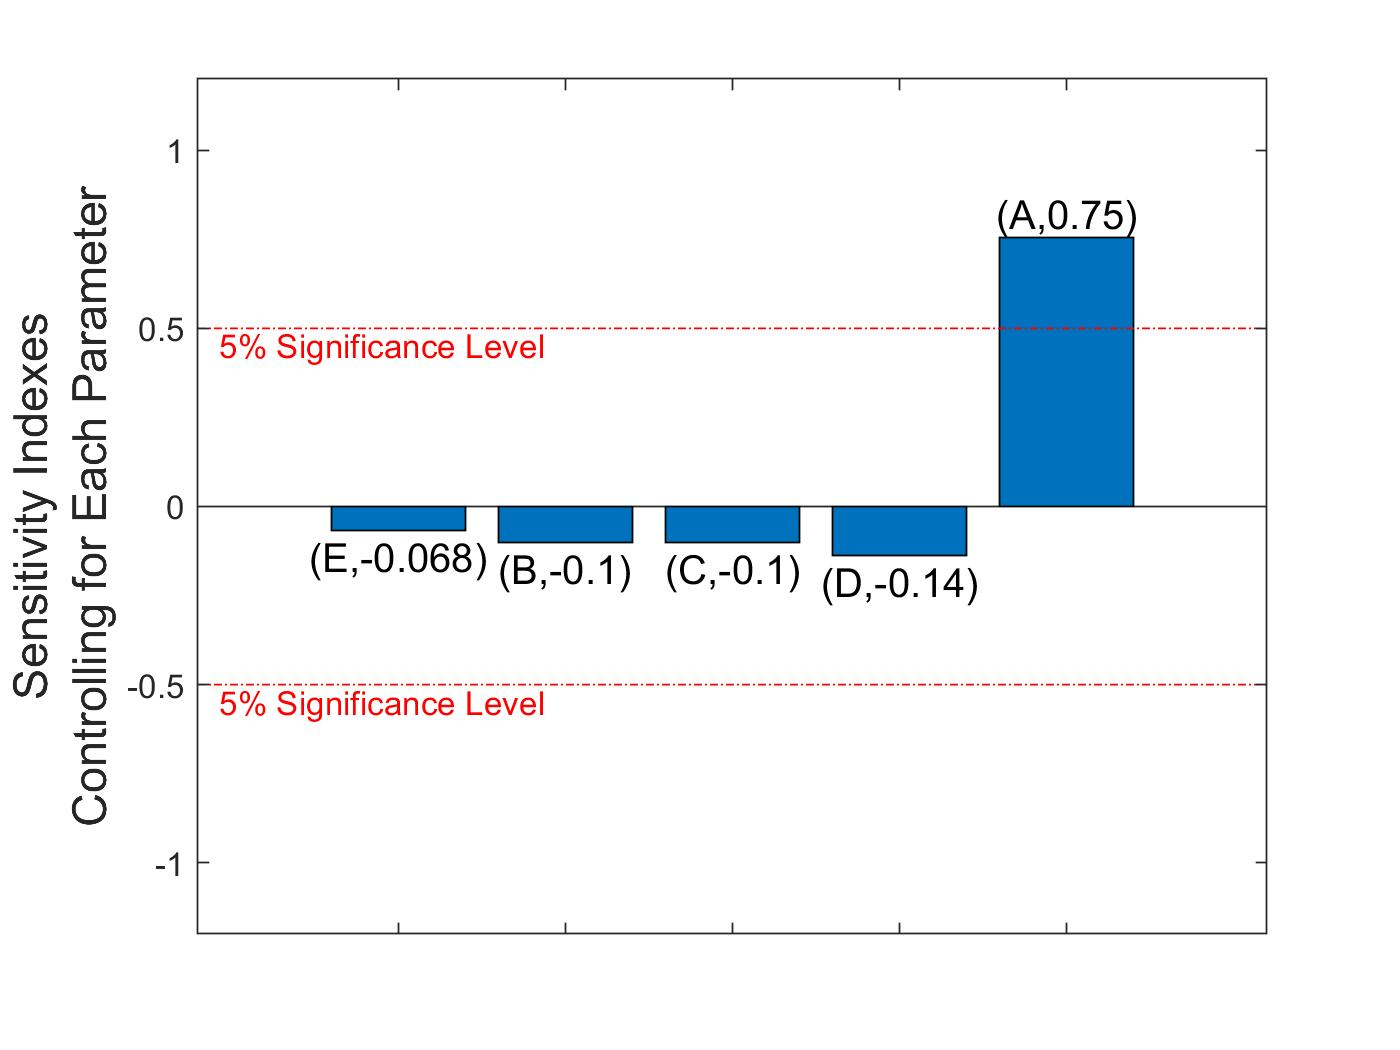
\includegraphics[width=\textwidth]{Zika_PE_figs/beta_h_PRCC.jpg}
         \caption{$\beta_h$ }
         \label{fig:betah_prcc}
     \end{subfigure}
      \hfill
     \begin{subfigure}[b]{0.45\textwidth}
         \centering
         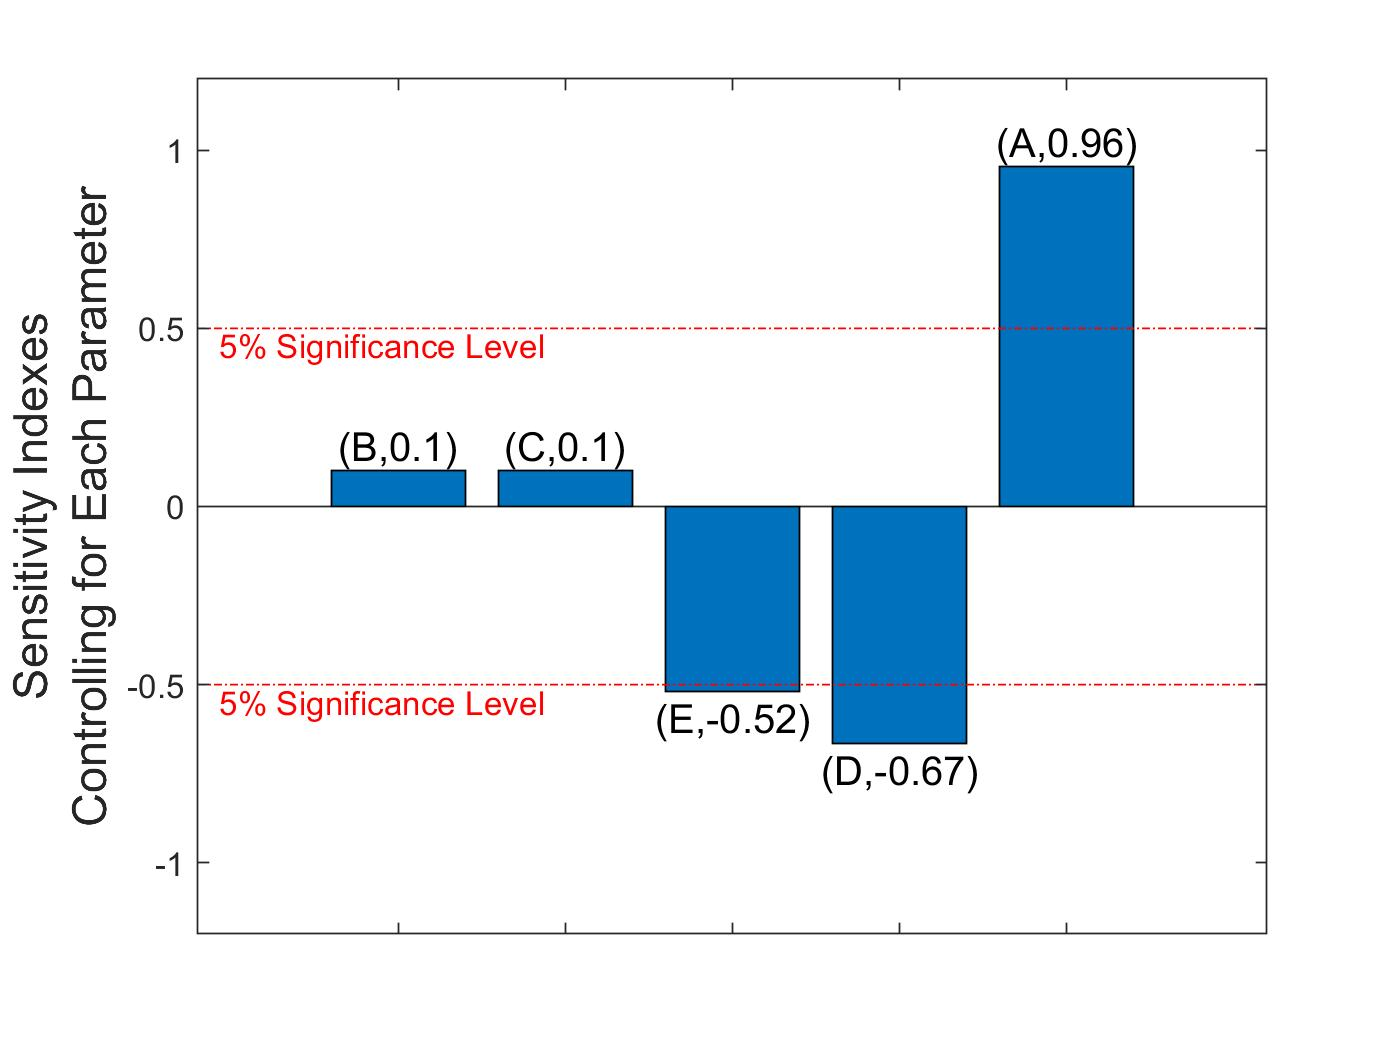
\includegraphics[width=\textwidth]{Zika_PE_figs/beta_V_PRCC.jpg}
         \caption{$\beta_V$}
         \label{fig:betav_prcc}
     \end{subfigure}
        
        \label{fig:PRCC}
\end{figure}

\section*{Discussion}
\paragraph{Limitations.} We assume that each region is isolated from the others during the calibration of the model for each region (that is, no movement of people or mosquitoes between the regions). No vertical transmission (since we simulate for only a year). No temperature dependence of mosquito-related processes. No vertical transmission.
\paragraph{Future work.} 

\section*{Conclusion}

\section*{Supporting information}

\paragraph*{S1 Fig.}
\label{S1_Fig}
{\bf Bold the title sentence.} Add descriptive text after the title of the item (optional).
\paragraph*{S1 File.}
\label{S1_File}
{\bf Lorem ipsum.}  Maecenas convallis mauris sit amet sem ultrices gravida. Etiam eget sapien nibh. Sed ac ipsum eget enim egestas ullamcorper nec euismod ligula. Curabitur fringilla pulvinar lectus consectetur pellentesque.

\paragraph*{S1 Video.}
\label{S1_Video}
{\bf Lorem ipsum.}  Maecenas convallis mauris sit amet sem ultrices gravida. Etiam eget sapien nibh. Sed ac ipsum eget enim egestas ullamcorper nec euismod ligula. Curabitur fringilla pulvinar lectus consectetur pellentesque.

\paragraph*{S1 Appendix.}
\label{S1_Appendix}
{\bf Lorem ipsum.} Maecenas convallis mauris sit amet sem ultrices gravida. Etiam eget sapien nibh. Sed ac ipsum eget enim egestas ullamcorper nec euismod ligula. Curabitur fringilla pulvinar lectus consectetur pellentesque.

\paragraph*{S1 Table.}
\label{S1_Table}
{\bf Lorem ipsum.} Maecenas convallis mauris sit amet sem ultrices gravida. Etiam eget sapien nibh. Sed ac ipsum eget enim egestas ullamcorper nec euismod ligula. Curabitur fringilla pulvinar lectus consectetur pellentesque.

\section*{Acknowledgments}

\nolinenumbers
\bibliographystyle{plos2015}
\bibliography{zika_ref}
\pagebreak
\appendix
\section{Data}
\begin{table}
    \centering
    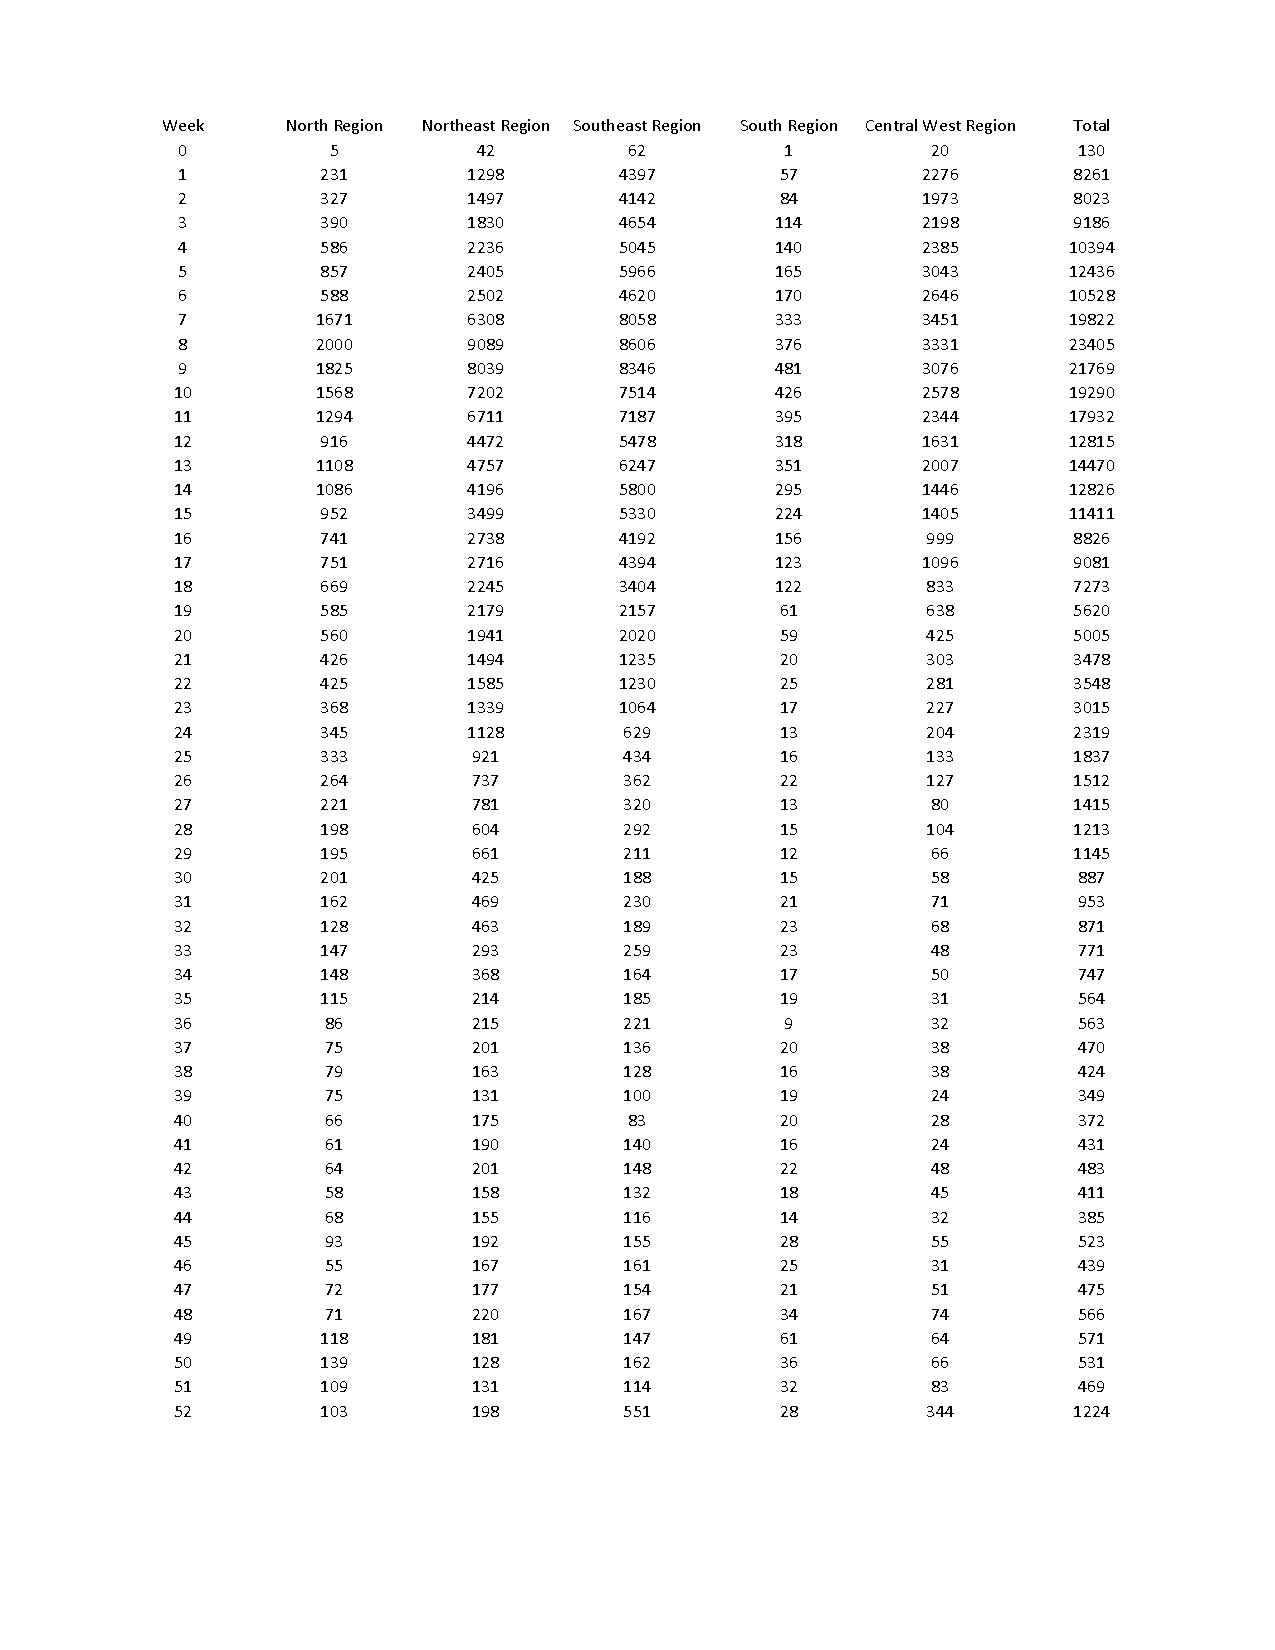
\includegraphics[height = 0.85\textheight,  trim = 2cm 4cm 2cm 4cm]{Zika_PE_figs/Brazil_zika_by_region.pdf}
    \caption{Brazil data. Source: \url{http://tabnet.datasus.gov.br/cgi/tabcgi.exe?sinannet/cnv/zikabr.def} (Accessed: March 2021)}
    \label{tab:zika_data}
\end{table}
\begin{figure}
     \centering
     \begin{subfigure}[b]{0.3\textwidth}
         \centering
         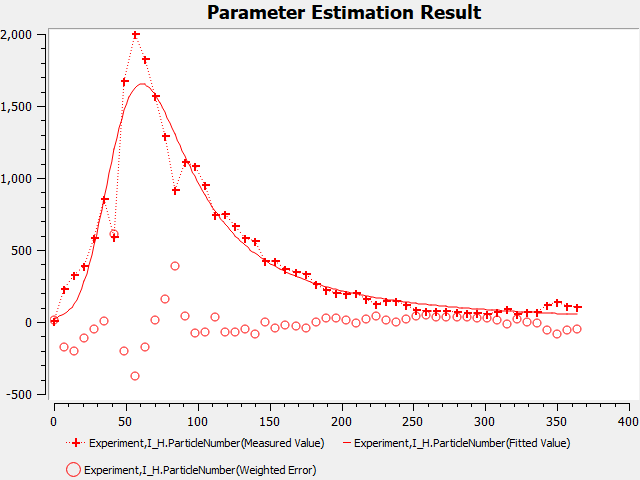
\includegraphics[width=\textwidth]{Zika_PE_figs/north_PE_0419.png}
         \caption{North}
         \label{fig:north_PE}
     \end{subfigure}
     \hfill
     \begin{subfigure}[b]{0.3\textwidth}
         \centering
         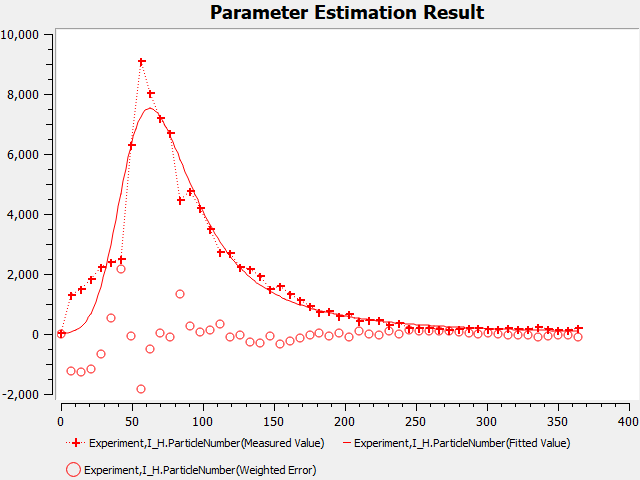
\includegraphics[width=\textwidth]{Zika_PE_figs/northeast_PE_0419.png}
         \caption{Northeast}
         \label{fig:NE_PE}
     \end{subfigure}
     \hfill
     \begin{subfigure}[b]{0.3\textwidth}
         \centering
         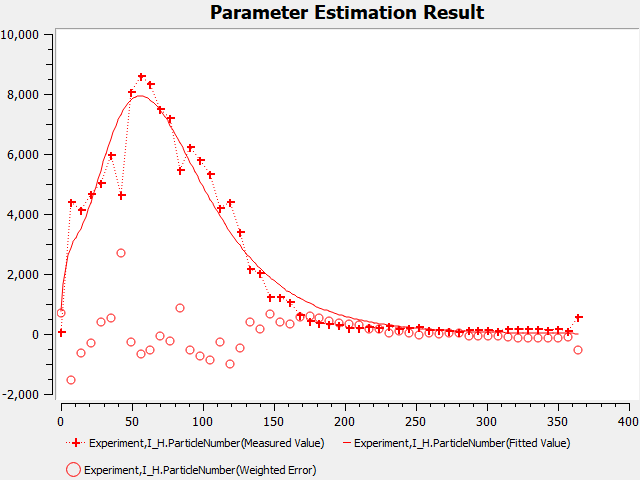
\includegraphics[width=\textwidth]{Zika_PE_figs/southeast_PE_0419.png}
         \caption{Southeast}
         \label{fig:SE_PE}
     \end{subfigure}
      \hfill
     \begin{subfigure}[b]{0.3\textwidth}
         \centering
         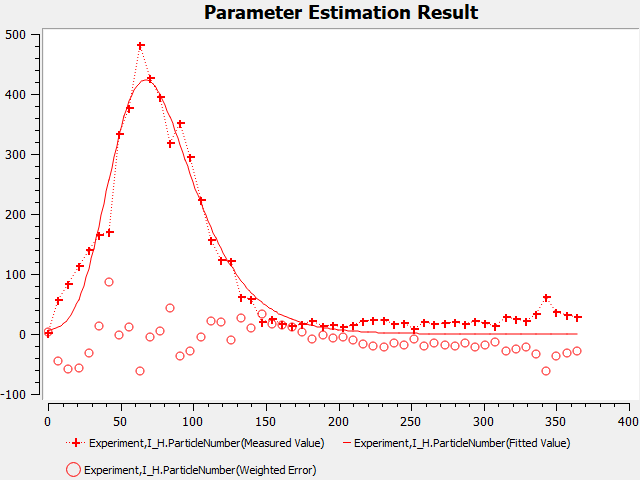
\includegraphics[width=\textwidth]{Zika_PE_figs/south_PE_0419.png}
         \caption{South}
         \label{fig:south_PE}
     \end{subfigure}
      \hfill
     \begin{subfigure}[b]{0.3\textwidth}
         \centering
         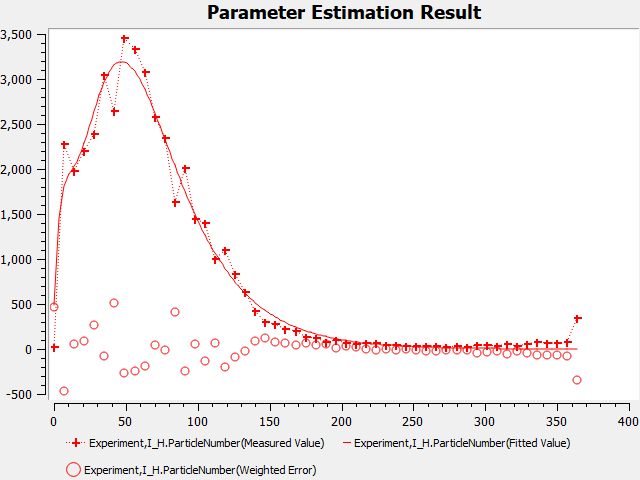
\includegraphics[width=\textwidth]{Zika_PE_figs/centralwest_PE_0419.png}
         \caption{Central West}
         \label{fig:CW_PE}
     \end{subfigure}
      \hfill
     \begin{subfigure}[b]{0.3\textwidth}
         \centering
         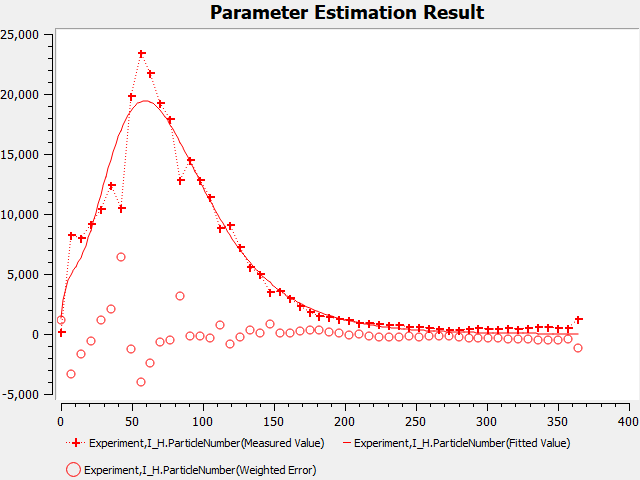
\includegraphics[width=\textwidth]{Zika_PE_figs/brazil_PE_0419.png}
         \caption{Brazil}
         \label{fig:brazil_PE}
     \end{subfigure}
        \caption{Model fit to data with parameters from Tables \ref{tab:zika_param_est} and \ref{tab:param-est-2}}
        \label{fig:PE_figs}
\end{figure}
\textbf{Best fit total vector population at equilibrium:}

North: 1.75968e+08

Northeast: 5.6751e+08

Southeast: 8.63e+08

South: 2.94e+08

Central West: 1.55982e+08

Brazil: 2.0516e+09
\end{document}